\chapter{LAB Session 02 -- Fully Differential Current-Mirror OTA}
\section{Schematic and Testbench Configuration}
\begin{figure}[H]
    \centering
    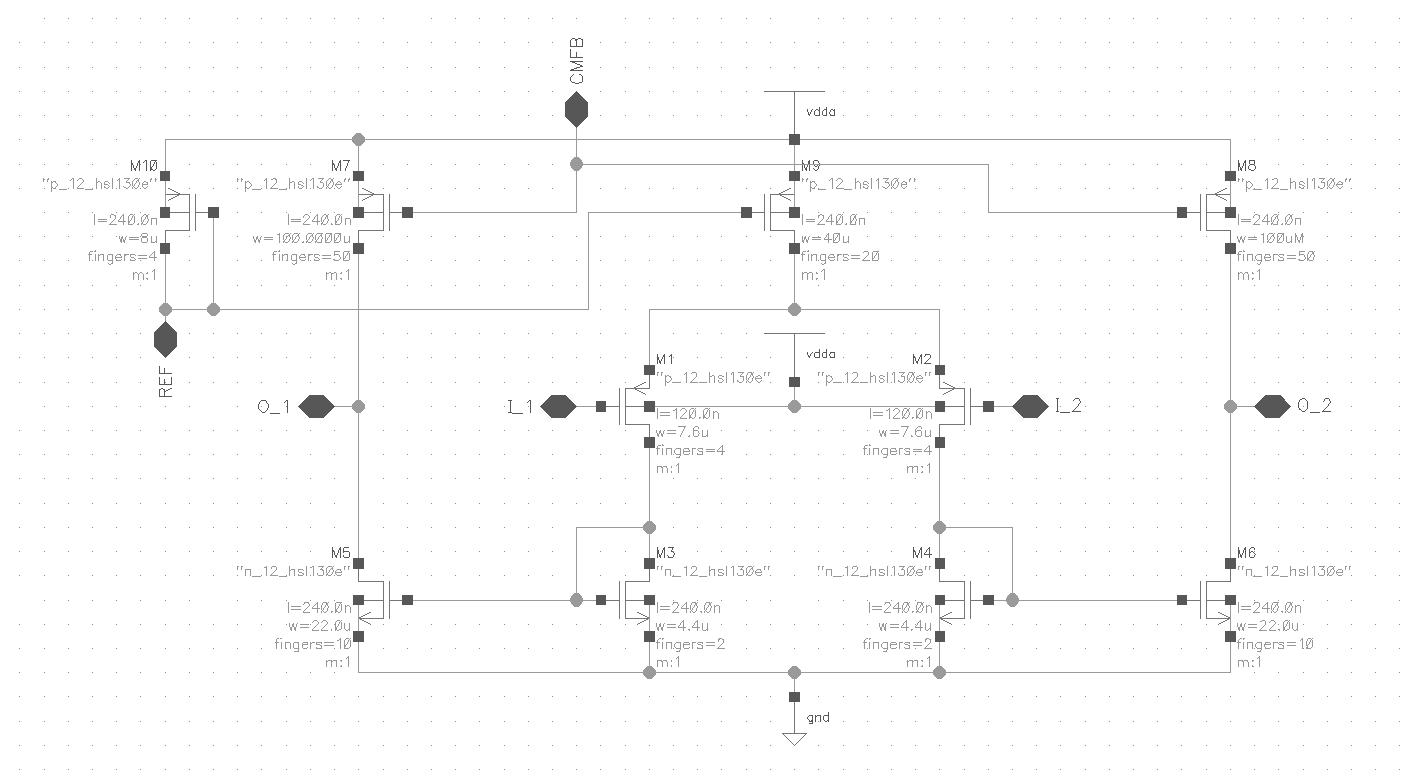
\includegraphics[width=1.0\linewidth]{imagespart2/schematics_OTA.png}
    \caption{Schematic}
\end{figure}
\begin{figure}[H]
    \centering
    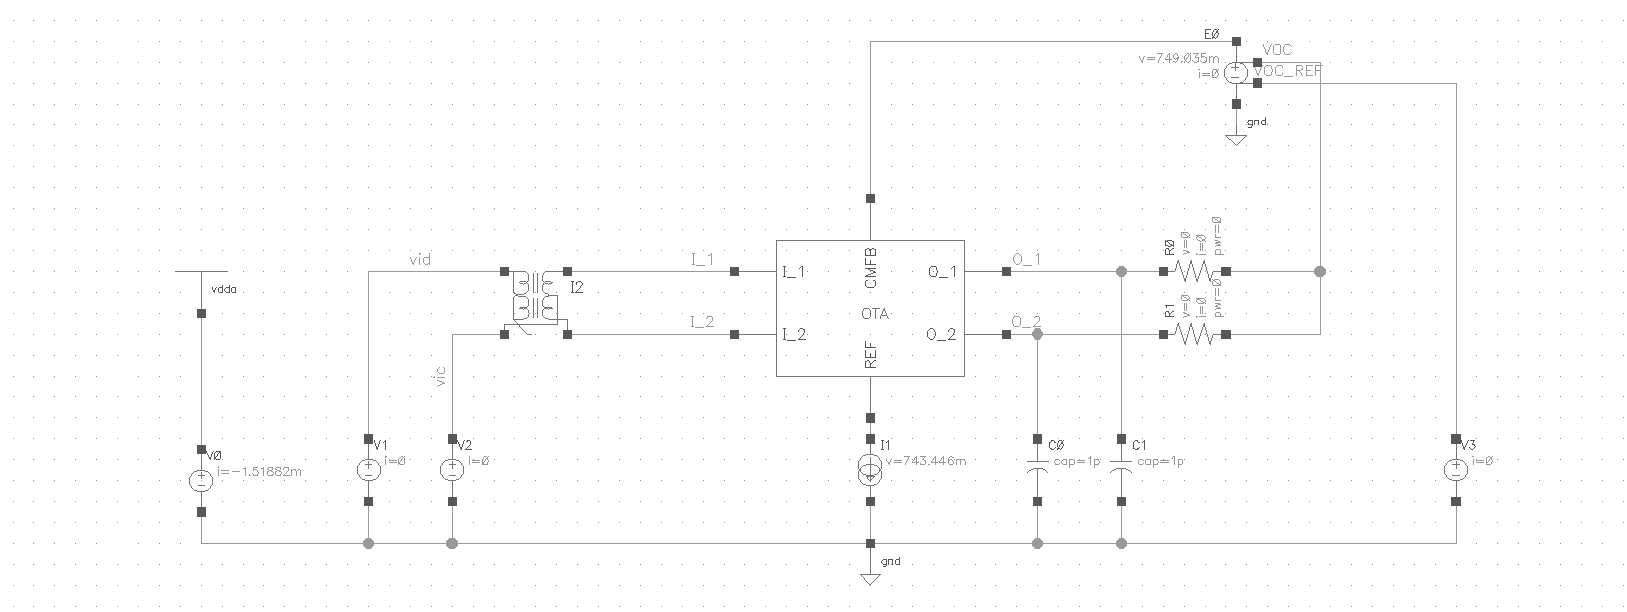
\includegraphics[width=1.0\linewidth]{imagespart2/schematics_tb.png}
    \caption{Testbench}
\end{figure}
\section{DC and Small-Signal Characterization}
\subsection{DC analysis}
\begin{figure}[H]
    \centering
    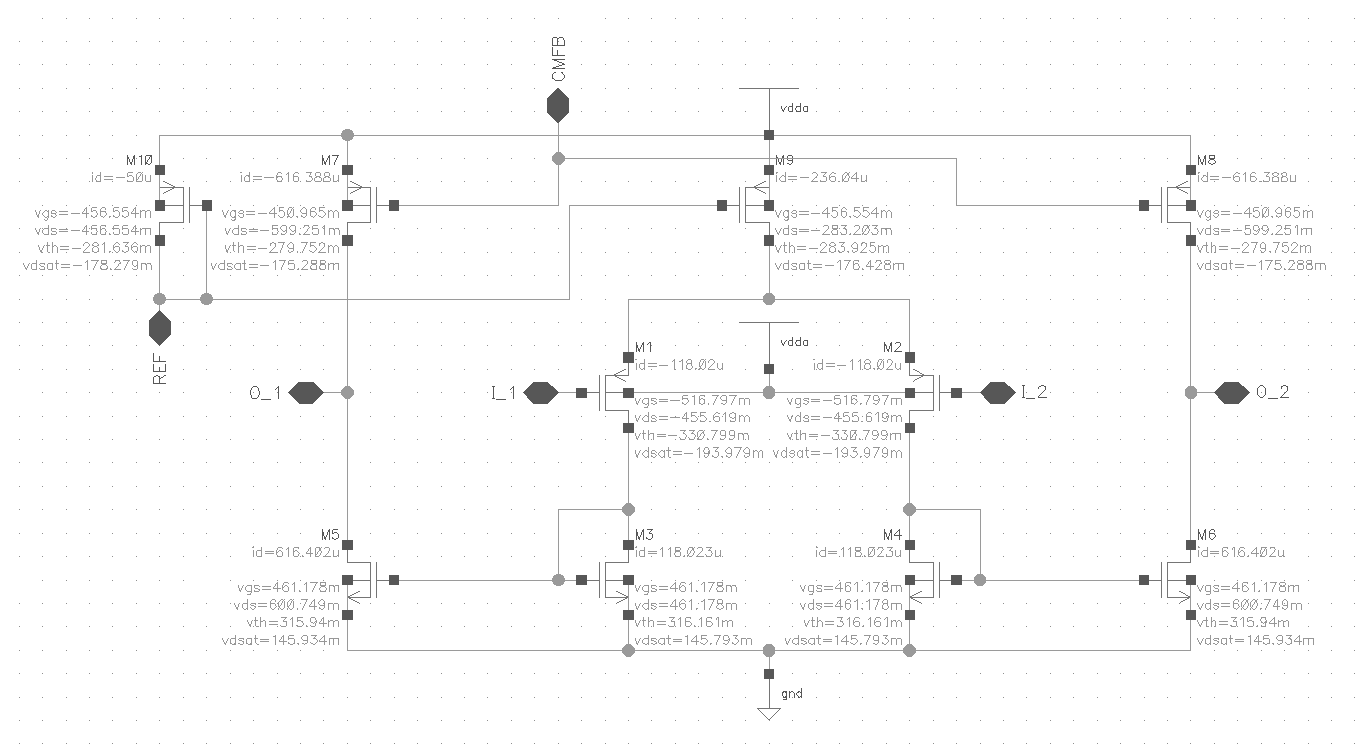
\includegraphics[width=1.0\linewidth]{imagespart2/OTA_OP.png}
    \caption{DC operating point}
\end{figure}


\begin{table}[H]
\centering
\caption{DC Operating Point Parameters of the OTA (Left Half-Circuit)}
\label{table:ota_op}
\begin{tabular}{|l|c|c|c|c|}
\hline
\textbf{Transistor} & \textbf{$|I_D|$ [$\mu$A]} & \textbf{$V_{DS}$ [mV]} & \textbf{$g_m$ [mS]} & \textbf{$r_o$ [k$\Omega$]} \\ \hline
M1  & 118.02  & 455.62 & 1.080   & 8.626  \\ \hline
M3  & 118.02 & 461.18 & 1.237 & 25.50 \\ \hline
M5  & 616.40 & 600.75 & 6.395 & 5.471  \\ \hline
M7  & 616.38 & 599.25 & 6.151 & 5.663 \\ \hline
M9  & 236.04 & 283.20 & 2.327 & 10.02   \\ \hline
M10 & 50 & 456.55 & 0.490 & 67.44 \\ \hline
\end{tabular}
\end{table}

\begin{figure}[H]
    \centering
    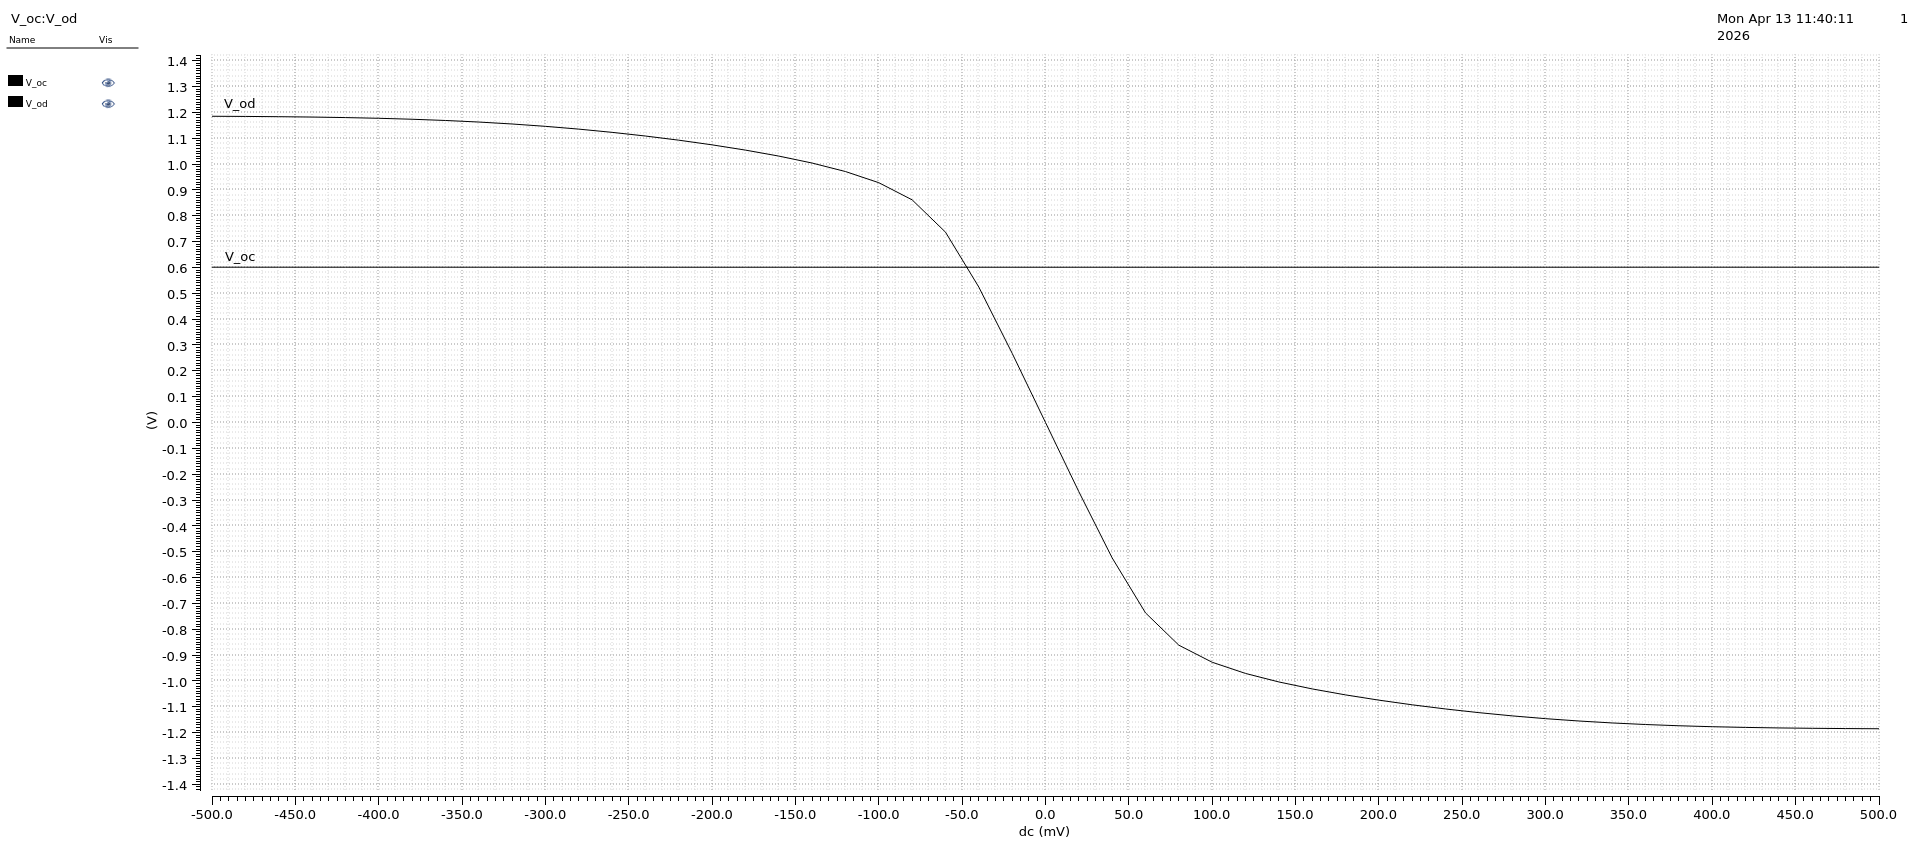
\includegraphics[width=1.0\linewidth]{imagespart2/V_oc_v_Vod.png}
    \caption{Differential output voltage $V_{OD}$ and common-mode output voltage $V_{OC}$ as functions of the differential input voltage $V_{ID}$.}
\end{figure}
\begin{figure}[H]
    \centering
    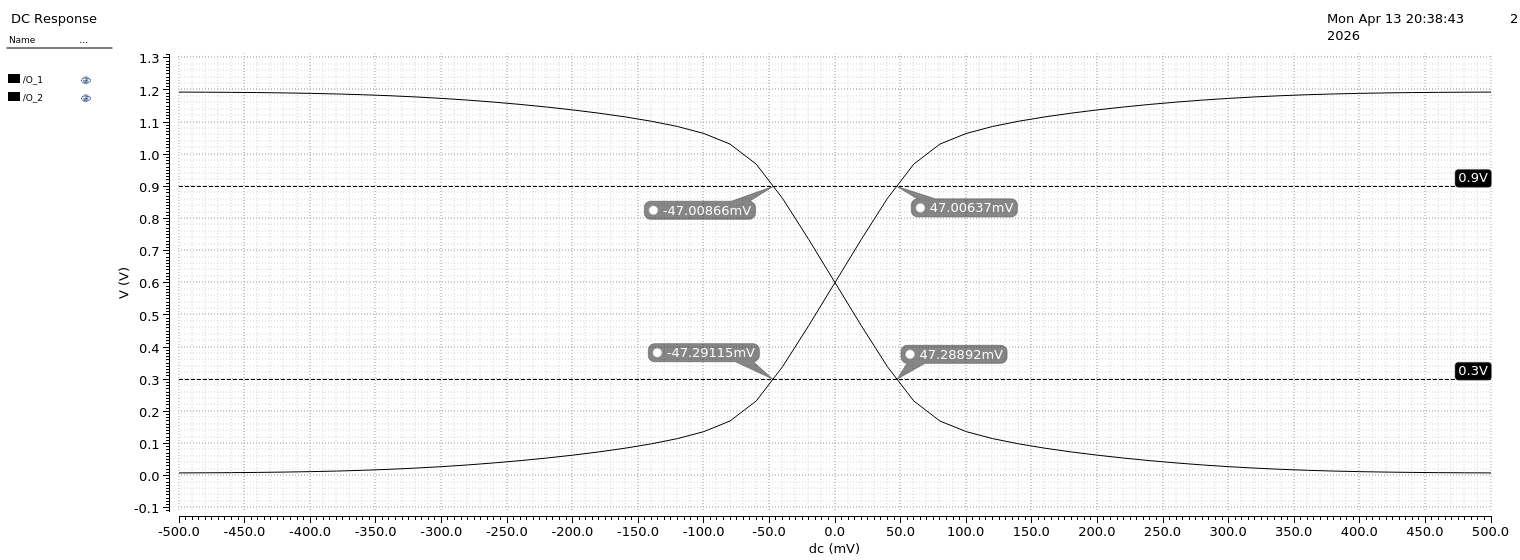
\includegraphics[width=1.0\linewidth]{imagespart2/Vo1_o2_id.png}
    \caption{Voltage outputs $V_{O1}$,$V_{O2}$ as functions $V_{ID}$.}
\end{figure}
\begin{figure}[H]
    \centering
    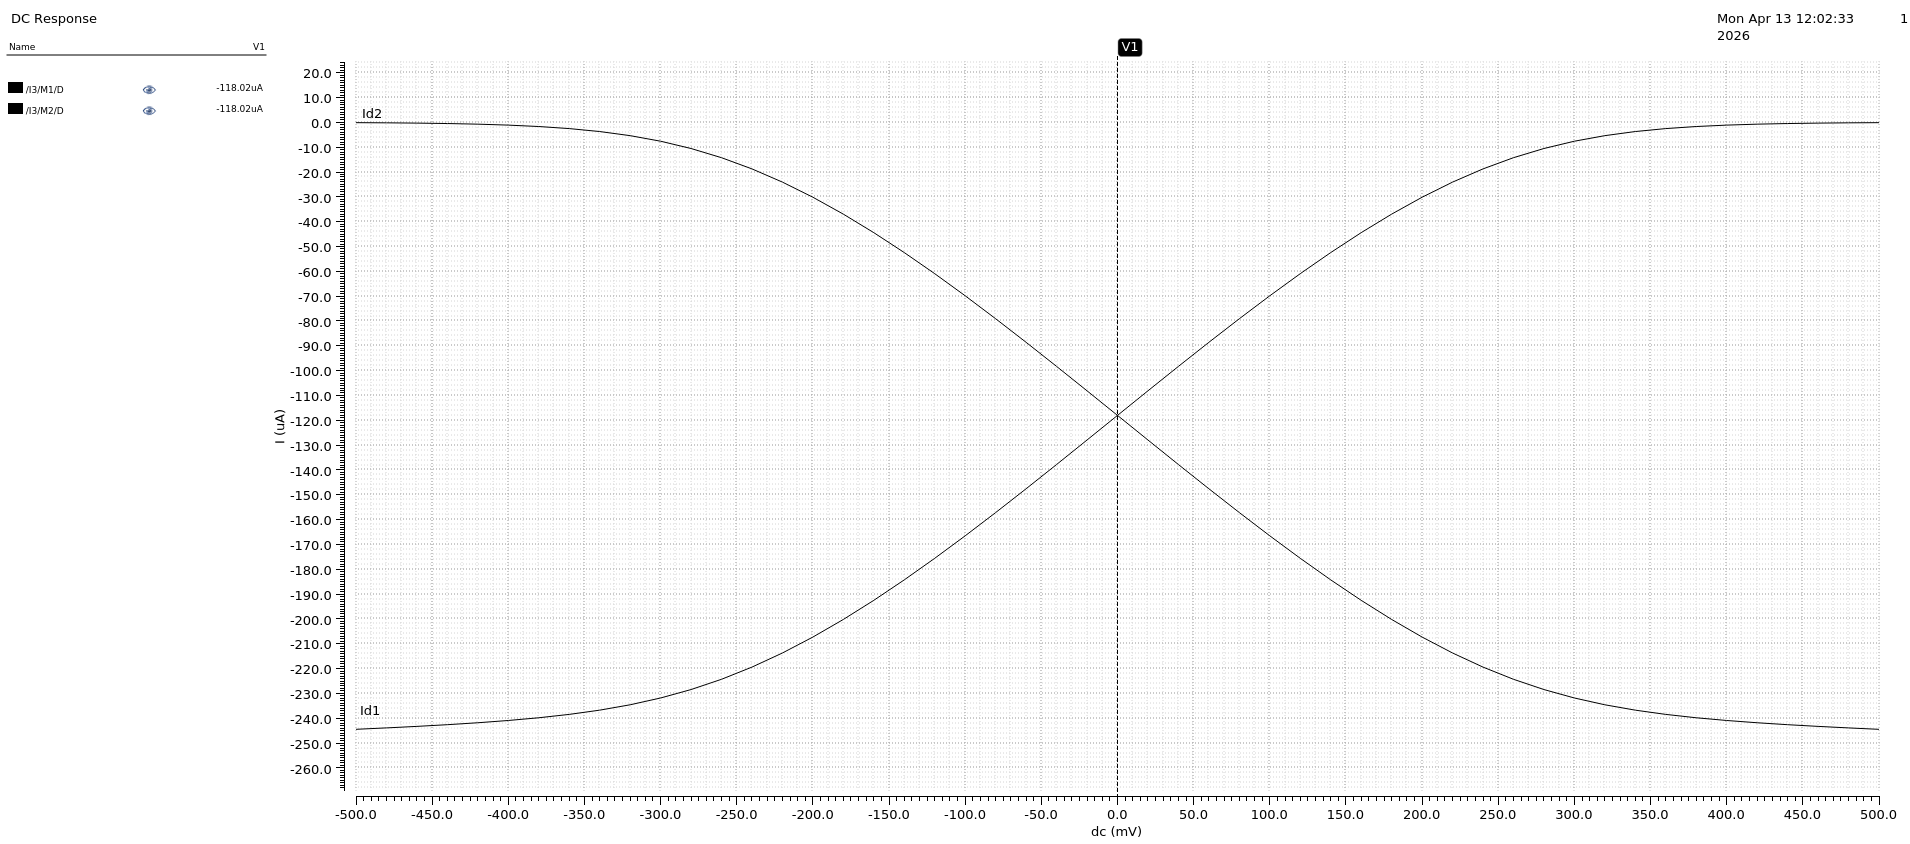
\includegraphics[width=1.0\linewidth]{imagespart2/Id1vId2.png}
    \caption{Differential pair currents as a function of $V_{ID}$.}
\end{figure}

\paragraph{Discussion of the differential-pair currents}
The simulated drain currents of the differential pair exhibit the expected current-steering behaviour. For large negative values of $V_{ID}$, most of the tail current flows through transistor M1, while the current in M2 becomes very small. Conversely, for large positive values of $V_{ID}$, the current is steered towards M2 and M1 is progressively turned off. Around $V_{ID}=0$, the two transistors conduct approximately the same current, corresponding to the balanced operating condition of the OTA.
\subsection{Differential mode ac analysis}
\begin{figure}[H]
    \centering
    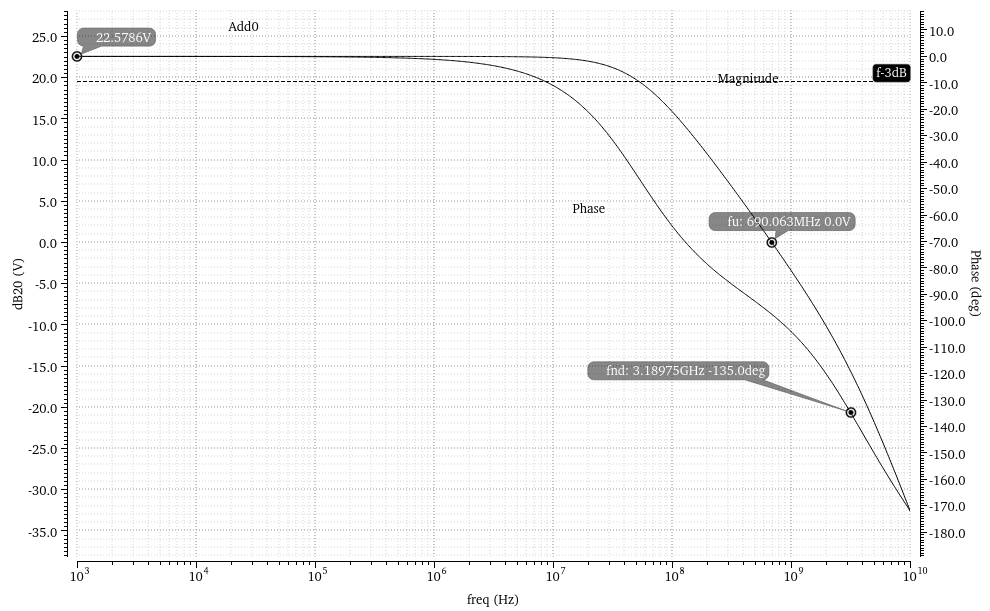
\includegraphics[width=1.0\linewidth]{imagespart2/differential_gain (1).png}
    \caption{Bode plot of magnitude and phase of the differential output voltage.}
\end{figure}


The differential-mode Bode plot has been analyzed by placing markers on both the magnitude and phase responses in order to extract the main performance parameters of the OTA. In particular, the low-frequency gain $A_{dd0}$, the $-3$ dB bandwidth $f_{-3\mathrm{dB}}$, and the unity-gain frequency $f_u$ have been identified from the magnitude response.

The extracted values are:

\begin{itemize}
    \item $A_{dd0}=22.58\,\mathrm{dB}$
    \item $f_{-3\mathrm{dB}}=52.28\,\mathrm{MHz}$
    \item $f_u=690.06\,\mathrm{MHz}$
\end{itemize}

The $-3$ dB bandwidth provides a good approximation of the dominant pole frequency:
\[
f_{dp}\approx f_{-3\mathrm{dB}}=52.28\,\mathrm{MHz}.
\]
Since the phase margin is large and the first non-dominant pole is located well above the unity-gain frequency, the gain-bandwidth product can be approximated as
\[
\mathrm{GBW}\approx f_u=690.06\,\mathrm{MHz}.
\]
The frequency of the first non-dominant pole was estimated from the phase response. A marker was placed at the frequency where the phase reaches approximately $-135^\circ$, corresponding to the point at which the second pole starts contributing significantly to the overall phase shift. This gives
\[
f_{nd}\approx 3.19\,\mathrm{GHz}.
\]
Since $f_{nd}\approx 4.6\,f_u$, the first non-dominant pole is sufficiently separated from the unity-gain frequency, confirming that the OTA behaves predominantly as a single-pole system around $f_u$.
\subsection{Common mode ac analysis}
\paragraph{Explanation for the very low value of the low-frequency
common-mode gain (and thus, very high CMRR)}
\begin{figure}[H]
    \centering
    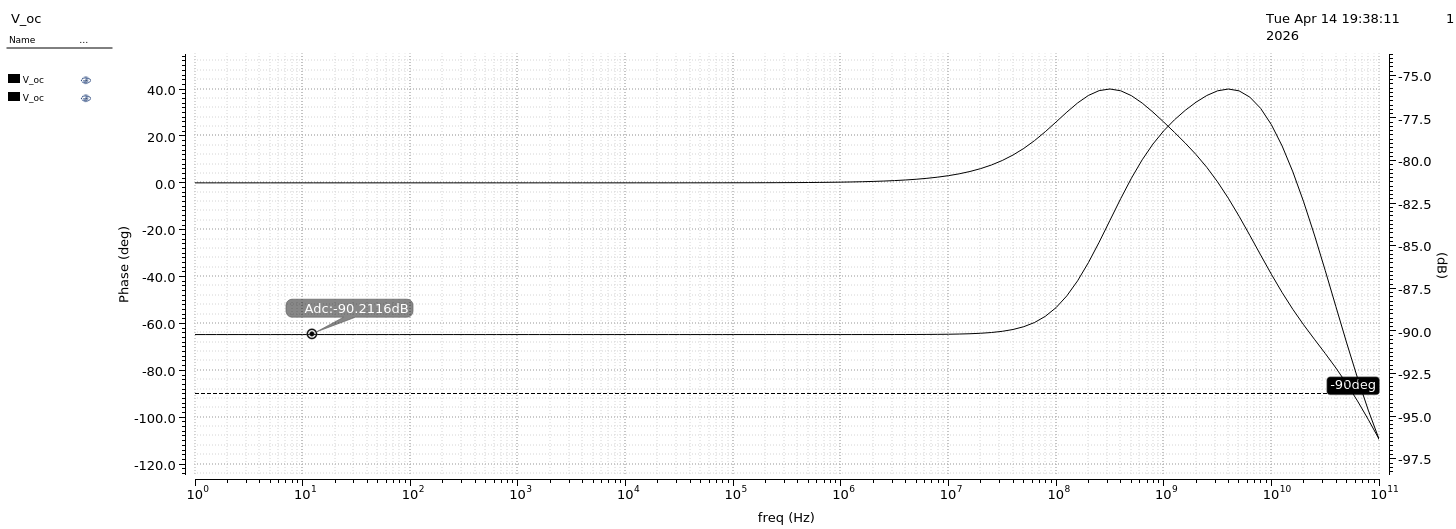
\includegraphics[width=1.0\linewidth]{imagespart2/Voc_gian_pahae.png}
    \caption{Bode plot of magnitude and phase of the common mode output voltage.}
\end{figure}
\paragraph{Discussion:}
The very low common-mode gain at low frequency is mainly due to the action of the Common-Mode Feedback (CMFB) loop. The CMFB senses the output common-mode voltage 
\[
V_{OC}=\frac{V_{O1}+V_{O2}}{2}
\]
and compares it with a reference value \(V_{OC,ref}\). Any deviation generates an error signal that is amplified and fed back to control the biasing of the output stage.

At low frequency, the CMFB loop has high gain, so it effectively forces
\[
V_{OC} \approx V_{OC,ref}
\]
independently of common-mode disturbances. As a result, variations in the input common-mode voltage produce only very small variations at the output, leading to a very low common-mode gain, and thus leading to a high CMRR.

\section{Estimation of the OTA Offset Voltage with a Monte Carlo Mismatch Simulation}


\begin{figure}[H]
    \centering
    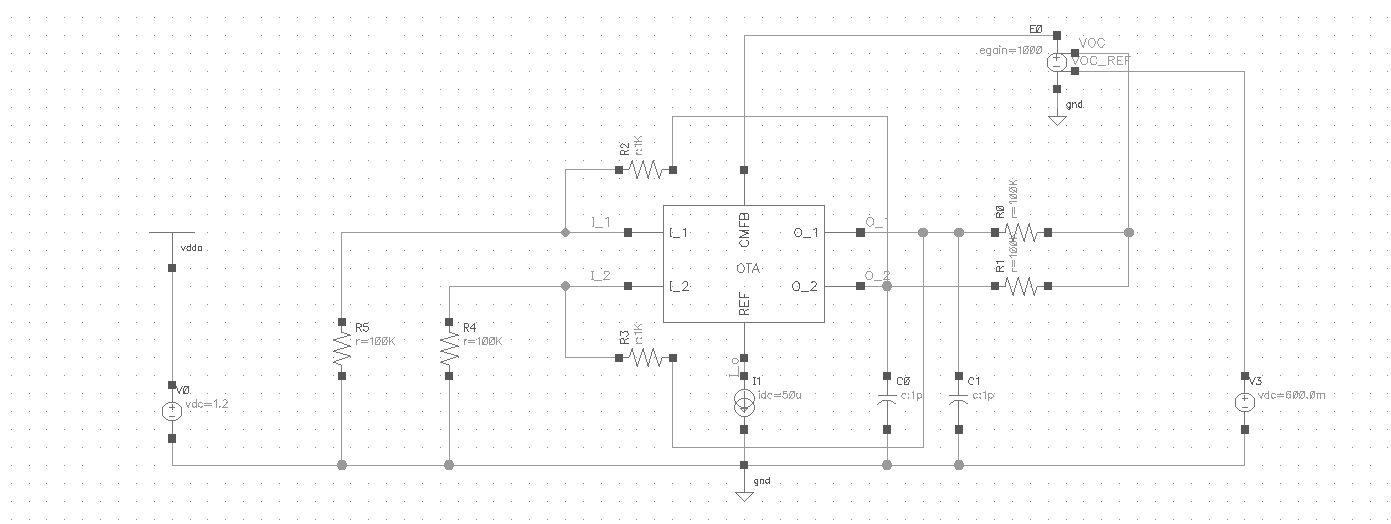
\includegraphics[width=1.0\textwidth]{imagespart2/ota_mirror_tb_schematic.png}
    \caption{Testbench used for the estimation of the OTA offset voltage.}
    \label{fig:vos_testbench}
\end{figure}
The OTA offset voltage was estimated by means of a Monte Carlo mismatch simulation including 100 runs. Using the feedback network shown in Fig.~\ref{fig:vos_testbench} and assuming $\beta A_{dd0} \gg 1$, the differential input voltage required to balance the output provides a good approximation of the input-referred mismatch voltage. Therefore, the OTA offset voltage can be estimated as

\[
V_{OS} \approx \sigma(V_{ID}).
\]

The distribution of $V_{ID}$ obtained from the Monte Carlo analysis is shown in Fig.~\ref{fig:hist_vid}. From the statistical data, the following standard deviation was extracted:

\[
\sigma(V_{ID}) =V_{OS}= 7.28\,\mathrm{mV}.
\]


\begin{figure}[H]
    \centering
    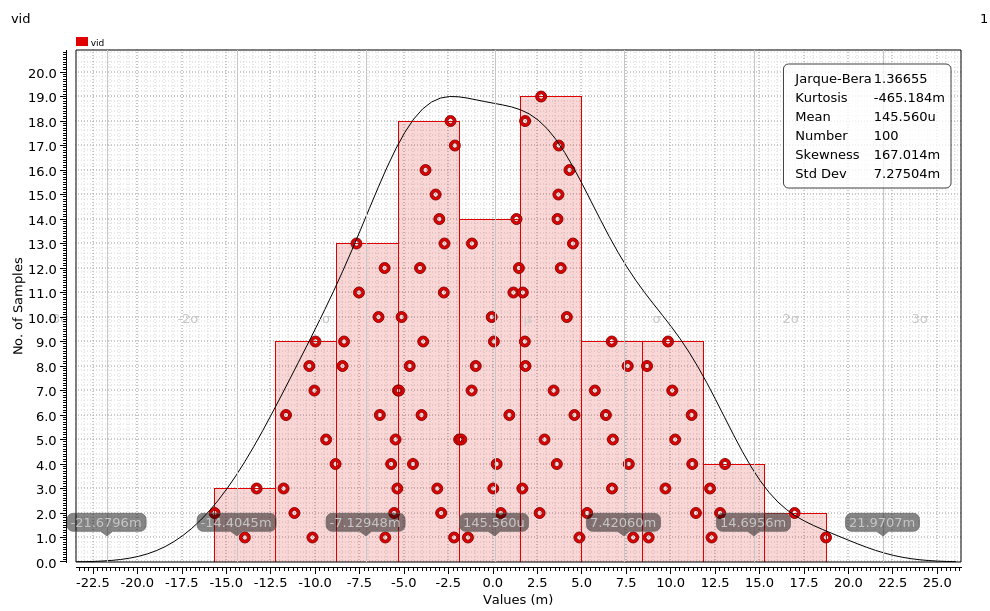
\includegraphics[width=1.0\textwidth]{imagespart2/Montecarlo Vid.png}
    \caption{Monte Carlo distribution of the differential input voltage $V_{ID}$.}
    \label{fig:hist_vid}
\end{figure}

\begin{figure}[H]
    \centering
    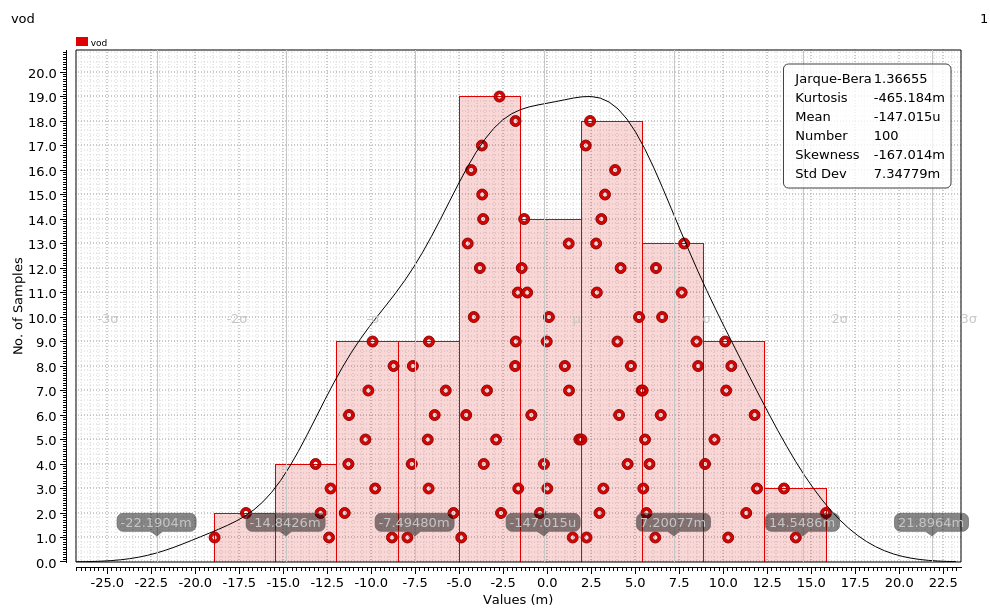
\includegraphics[width=1.0\textwidth]{imagespart2/Montecarlo Vod.png}
    \caption{Monte Carlo distribution of the differential output voltage $V_{OD}$.}
    \label{fig:hist_vod}
\end{figure}
\section{Redesign of the OTA to meet specifications}
The OTA was initially designed following the procedure described in the previous sections, targeting a gain-bandwidth product of $1\,\mathrm{GHz}$. However, AC simulations yielded a unity-gain frequency of approximately $600\,\mathrm{MHz}$, indicating that the simplified long-channel design equations overestimated the achievable performance.

To compensate for these non-ideal effects, the same sizing procedure was repeated using a more conservative target value

\[
GBW_{target}=1.6\,\mathrm{GHz}.
\]

This led to the following design parameters:

\[
G_m \approx 10.05\,\mathrm{mS},
\qquad
R_o \approx 3.96\,\mathrm{k}\Omega,
\]
with bias currents
\[
I_{D1}=I_{D2}\approx188\,\mu\mathrm{A},
\qquad
I_{B1}\approx376\,\mu\mathrm{A},
\qquad
I_{B2}\approx752\,\mu\mathrm{A}.
\]

The corresponding transistor dimensions were then calculated according to the adopted design methodology. In particular, the input differential pair dimensions were initially obtained as

\[
W_1=W_2=20\,\mu\mathrm{m},
\qquad
L_1=L_2=120\,\mathrm{nm}.
\]

Although this redesigned OTA exhibited a significant improvement with respect to the initial implementation, the simulated gain-bandwidth product was still slightly below the required specification of $1\,\mathrm{GHz}$.

Therefore, a final optimization step was performed by increasing the width of the input differential pair transistors from $20\,\mu\mathrm{m}$ to $33\,\mu\mathrm{m}$. This modification increases the transconductance $g_{m1}$ of the input stage by reducing its overdrive voltage, while still keeping the devices in strong inversion. As a consequence, the gain-bandwidth product is increased without significantly altering the bias currents, output resistance, or operating point of the OTA.

The final transistor dimensions adopted for the implementation are summarized in Table~\ref{tab:final_sizing2}.

\begin{table}[H]
\centering
\caption{Final transistor dimensions after optimization.}
\label{tab:final_sizing2}

\begin{tabular}{|c|c|c|}
\hline
\textbf{Transistor} & \textbf{W [$\mu$m]} & \textbf{L [nm]} \\ \hline
M1, M2 & $20 \xrightarrow{} 33$ & 120 \\ \hline
M3, M4 & 3.6 & 450 \\ \hline
M5, M6 & 14.4 & 450 \\ \hline
M7, M8 & 52 & 450 \\ \hline
M9 & 26 & 450 \\ \hline
M10 & 3.6 & 450 \\ \hline
\end{tabular}

\end{table}
\section{Final Design Verification}

\begin{figure}[H]
    \centering
    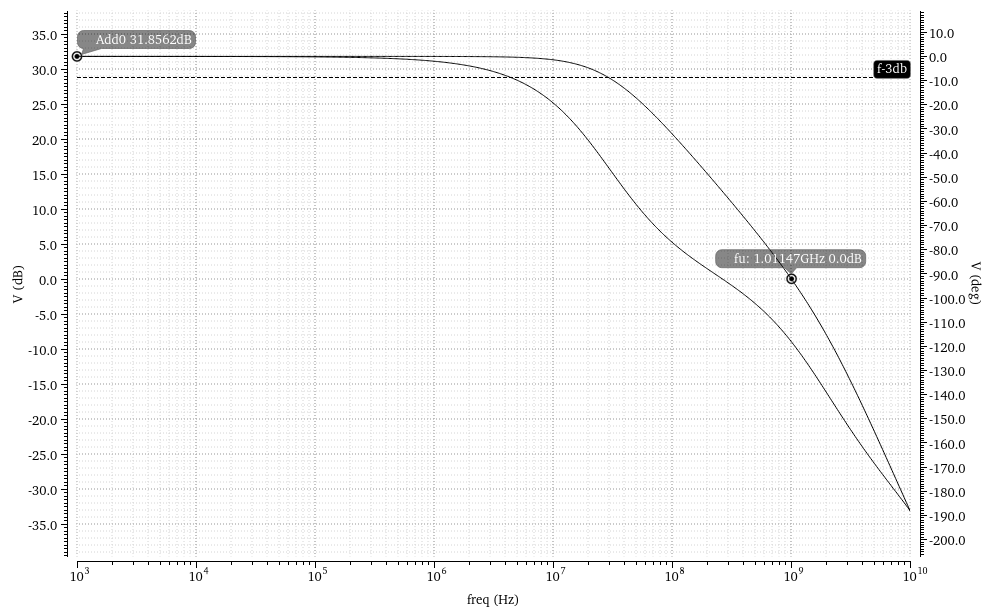
\includegraphics[width=\linewidth]{imagespart2/final_differential_gain.png}
    \caption{Differential-mode Bode plot of the final OTA design.}
    \label{fig:final_bode}
\end{figure}

The performance of the optimized OTA was verified through AC analysis. The differential-mode Bode plot reported in Fig.~\ref{fig:final_bode} shows that the final design successfully meets the assigned gain and bandwidth specifications.

The extracted values are:

\begin{itemize}
    \item $A_{dd0} \approx 31.86\,\mathrm{dB}$
    \item $GBW \approx 1.01\,\mathrm{GHz}$
\end{itemize}

The low-frequency gain exceeds the required specification of $30\,\mathrm{dB}$, while the unity-gain frequency is slightly above the target value of $1\,\mathrm{GHz}$. The increase of the input-pair width successfully enhanced the transconductance of the OTA, resulting in the desired improvement of the gain-bandwidth product without compromising the stability of the circuit.

\begin{figure}[H]
    \centering
    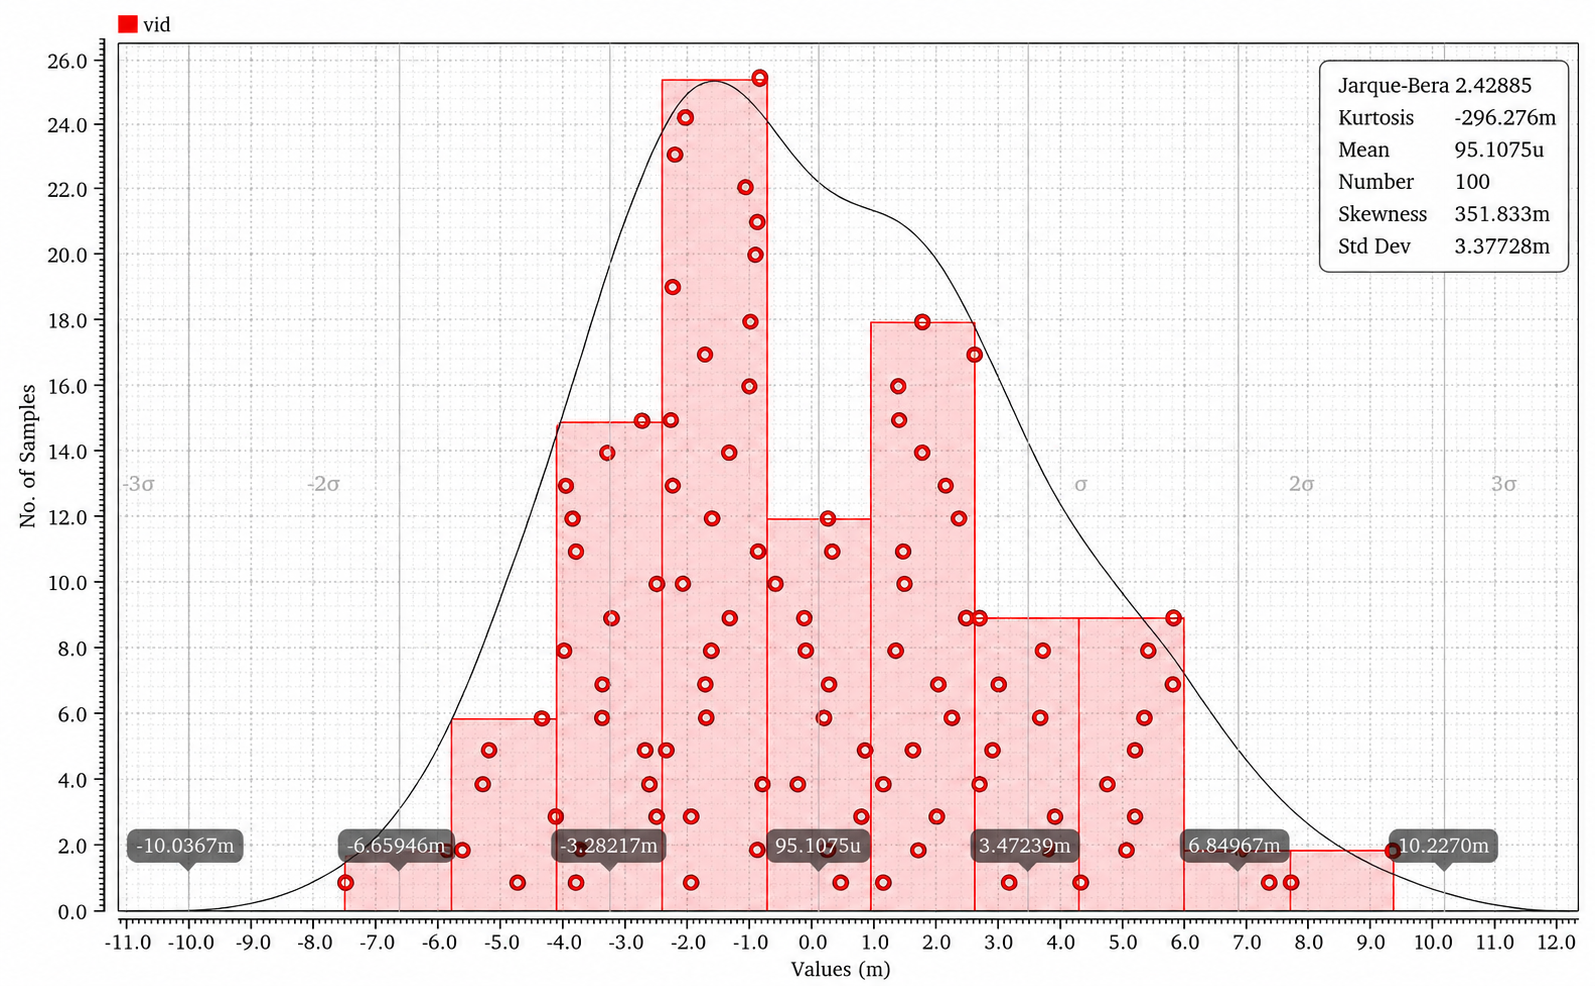
\includegraphics[width=\linewidth]{imagespart2/final_montecarlo_corretta.png}
    \caption{Monte Carlo distribution of the input-referred differential voltage $V_{ID}$ for the final OTA design.}
    \label{fig:final_mc}
\end{figure}

To verify the offset-voltage specification, a Monte Carlo mismatch simulation with $N=100$ runs was performed. The resulting distribution of the differential input voltage required to balance the output is shown in Fig.~\ref{fig:final_mc}.

From the statistical analysis, the standard deviation of the distribution was found to be

\[
\sigma(V_{ID}) =V_{OS}= 3.38\,\mathrm{mV}.
\]
\begin{table}[H]
\centering
\caption{Final specification verification.}
\label{tab:final_results}

\begin{tabular}{|c|c|c|c|}
\hline
\textbf{Parameter} & \textbf{Specification} & \textbf{Simulated} \\ \hline
$A_{dd0}$ & $>30\,\mathrm{dB}$ & $31.86\,\mathrm{dB}$  \\ \hline
GBW & $\geq1\,\mathrm{GHz}$ & $1.01\,\mathrm{GHz}$  \\ \hline
$V_{OS}$ & $<4\,\mathrm{mV}$ & $3.38\,\mathrm{mV}$  \\ \hline
\end{tabular}

\end{table}

